\documentclass[assignment03_Solutions]{subfiles}

\IfSubStr{\jobname}{\detokenize{Solutions}}{\toggletrue{solutions}}{\toggletrue{solutions}}

\fancypagestyle{firstpage}

{\rhead{Assignment 3 \linebreak \textit{Version: \today}}}

\title{Assignment 3: Fairness, Maximum Likelihood Estimation, and Text Classification}
\author{Machine Learning}
\date{Fall 2019}
\invalidatemargin

\begin{document}

\maketitle
\thispagestyle{firstpage}


\begin{learningobjectives}
\bi
\item TODO
\ei
\end{learningobjectives}

\section{Bayesian Networks and Algorithmic Fairness}


In assignment 1 of this module we discussed how Bayesian methods can be used to reason about algorithmic fairness.  We've just had some lengthy discussions about fairness within the context of the Compas algorithm.  We touched upon some of the limitations of statistically based notions of fairness.  Nevertheless, they do have a potential role to play, and you should know what the most common definitions of fairness are and what assumptions they make.

As context for the reading and to help us have common notation, suppose we have the following random variables.

\bi
\item $R$ is a prediction generated by our algorithm.
\item $A$ is a sensitive attribute
\item $Y$ is the thing we're trying to predict (we want $R = Y$ if we are predicting accurately)
\ei

\begin{externalresources}[(30 minutes)]
Read \href{https://fairmlbook.org/classification.html}{Fairness and Machine Learning Chapter 2}.  Start at the section \emph{Formal non-discrimination criteria} and read up to (but not including) the section \emph{Calibration and sufficiency}.
\begin{notice}
\bi
\item Don't get hung up on the \href{https://en.wikipedia.org/wiki/Receiver_operating_characteristic}{ROC curves}.  We can certainly discuss this on NB, but it is not required to understand what is going on here.  The presentation earlier in the linked reading is also pretty clear.
\item The notation they use in this reading for conditional independence is an upside down T with only one line (instead of our notation, $\condindep$).
\ei
\end{notice}
\end{externalresources}


\begin{exercise}[(5 minutes)]
Thinking back to the COMPAS example, which definition of fairness given in the reading was Propublica using?  Which definition of fairness was Northpointe using?

\begin{boxedsolution}
\bi
\item Northpointe is using sufficiency $Y \condindep A~|~R$.  You'll notice that in the reading they say that sufficiency is the same thing as matching positive and negative predictive value for all values of the protected attribute.
\item Propublica is using separation $R \condindep A~|~Y$.  This fairness principle requires the false positive and true positive rates to be the same across for all values of the protected attribute.
\ei
\end{boxedsolution}
\end{exercise}

TODO: possibly present the data from COMPAS in \href{https://colab.research.google.com/drive/1HMX0GJAF0PcCn6INfCoeqNOASJri_V_s}{a notebook}.

\section{Maximum Likelihood Parameter Estimation for Discrete Models}
Last assignment, we met the Na\"ive Bayes model.  As a motivating example, we presented a Bayesian Network (BN) for the Titanic Dataset that modeled three features (\emph{male}, \emph{is young}, and \emph{fare class}) being generated by whether or not the passenger survived.  Here is the BN corresponding to this model.

\begin{center}
\includegraphics[width=0.8\linewidth]{../02/figures/titanicbn}
\end{center}

Last assignment, we described how we determined the parameters in the conditional probability tables.
\begin{quote}
``The probabilities in this BN were computed by looking at the training set and counting the appropriate passengers that fell into each category.  For instance, to compute $p(\mathcal{Y}|\mathcal{S})$ since $p(\mathcal{Y}|\mathcal{S}) = \frac{p(\mathcal{Y}, \mathcal{S})}{p(\mathcal{S})}$, we can approximate this probability by counting the number of passengers under 5 who survived and dividing by the total number who survived (note that there are some subtle and important modifications to this method of fitting these probabilities that we'll discuss in the next assignment).  This process was repeated for each conditional probability.  Since we assume that all of the features are conditionally independent given the output ($\mathcal{S}$ in this case), this process is done independently for each feature.''
\end{quote}

While this (hopefully) seems quite logical, it helps to be rigorous about \emph{why} these are the right probabilities to fit given the training data.  In this section, we'll go over the math behind determining these probabilities.  The goal will be to provide a general outline of a process for fitting parameters of a BN.  We'll do so by analyzing the Na\"ive Bayes model in particular to help you get the ``recipe'' for how this works.

\subsection{Formalizing the Problem}
We can think of the numbers in the conditional probability tables as the parameters of our Bayesian Network.  In order to compute sensible values for those parameters, we're going to choose the parameters values that agree as closely as possible with a set of training data.  At a conceptual level this strategy should feel pretty familiar.  In the last module, we did this again and again by tuning model parameters to accurately predict the training outputs as a function of the training inputs (last module the parameters were typically weights of a neural network or a logistic regression model).

Suppose we are given $n$ training data points $\mathbf{x_1}, \mathbf{x_2}, \ldots, \mathbf{x_n}$.  In the case of the titanic dataset $\mathbf{x_i}$ would be a four-dimensional vector consisting of whether the passenger survived ($\mathcal{S}$), the passenger's fare class ($\mathcal{C}$), whether the passenger was male ($\mathcal{M}$), and whether the passenger was under the age of 5 ($\mathcal{Y}$).  Further, suppose our model is parameterized by parameters $\mathbf{\Theta}$, which provide the necessary information to compute the probability of any input $\mathbf{x}$.  In other words, our model can compute $p(\mathbf{x_i} | \mathbf{\Theta})$ for any of the training points (or any other possible input for that matter).

\begin{understandingcheck}
In the case of the Titanic model, what would the parameters $\mathbf{\Theta}$ represent? (check solutions for the answer).
\begin{boxedsolution}
The parameters in this case would represent all of the entries in the conditional probability tables in the BN.  For example, the parameters would encode $p(\mathcal{S})$, $p(\mathcal{M}|\mathcal{S})$, etc.
\end{boxedsolution}
\end{understandingcheck}

Given the our model of $p(\mathbf{x_i}|\mathbf{\Theta})$, we would now like to figure out the best parameters, $\mathbf{\Theta}^\star$ based on our training data.  To do this, we can use the technique of maximum likelihood estimation (MLE).  The maximum likelihood estimate of the parameters is given by the following formula.

\begin{align}
\mathbf{\Theta^\star} &= \argmax_{\mathbf{\Theta}} p(\mathbf{x_1}, \mathbf{x_2}, \ldots \mathbf{x_n} | \mathbf{\Theta}) \label{eq:mle}
\end{align}

This equation is known as maximum likelihood estimation because: (a) it involves a maximization and (b) it is a likelihood (probability of data given a hypothesis or model).  Intuitively, Equation~\ref{eq:mle} captures the idea that we should choose the model parameters that makes the observed training data as likely as possible under our model.

\subsection{Simplifications to Equation~\ref{eq:mle}}

It may seem that computing the probability in Equation~\ref{eq:mle} would be quite difficult.   While in some cases it can be, there are some simplifying assumptions that we can apply to make our lives easier.  One of the most common assumptions is that the training data points are conditionally independent given $\mathbf{\Theta}$ (that is $\mathbf{x_i} \condindep \mathbf{x_j}~|~\mathbf{\Theta}$ for all $i \neq j$).  This is known as the \href{https://en.wikipedia.org/wiki/Independent_and_identically_distributed_random_variables}{independently and identically distributed (i.i.d.) assumption}.

\begin{understandingcheck}
TODO: What does this mean?  are $\mathbf{x_i} \condindep \mathbf{x_j}$ for $i \neq j$ (without conditioning on $\mathbf{\Theta}$?  Make a conceptual argument to justify your answer.
\end{understandingcheck}

If we apply the i.i.d. assumption to Equation~\ref{eq:mle}, we derive the following equation.

\begin{align}
\mathbf{\Theta^\star} &= \argmax_{\mathbf{\Theta}} p(\mathbf{x_1} |  \mathbf{\Theta}) p(\mathbf{x_2} | \mathbf{\Theta}) \ldots p(\mathbf{x_n} | \mathbf{\Theta}) \label{eq:mleiid}
\end{align}

To things even easier, we can apply a log without changing the $\argmax$.  This works because $\log$ is a monotonic (continuously increasing) function, so $\argmax_x f(x) = \argmax_x \log  f(x) $).


\begin{align}
\mathbf{\Theta^\star} &= \argmax_{\mathbf{\Theta}} \log \left ( p(\mathbf{x_1} |  \mathbf{\Theta}) p(\mathbf{x_2} | \mathbf{\Theta}) \ldots p(\mathbf{x_n} | \mathbf{\Theta})  \right) \nonumber \\
&=  \argmax_{\mathbf{\Theta}} \sum_{i=1}^n \log p(\mathbf{x_i} |  \mathbf{\Theta})  \label{eq:mleiidlog}
\end{align}

The importance of applying the log might not be apparent yet, but it actually did some useful work.  Specifically, it broke apart our probability into multiple components (one for each data point).  We can now optimize the sum of a bunch of functions rather than the product (which turns out to be much easier).  We'll see how this plays out in the next section.

\subsection{Maximum Likelihood Estimation for Na\"ive Bayes}

In this section you'll be applying the technique of MLE to the Na\"ive Bayes algorithm.

\vspace{1em}
\begin{exercise}[(60 minutes)]
The BN for the Na\"ive Bayes model is shown below.

\begin{center}
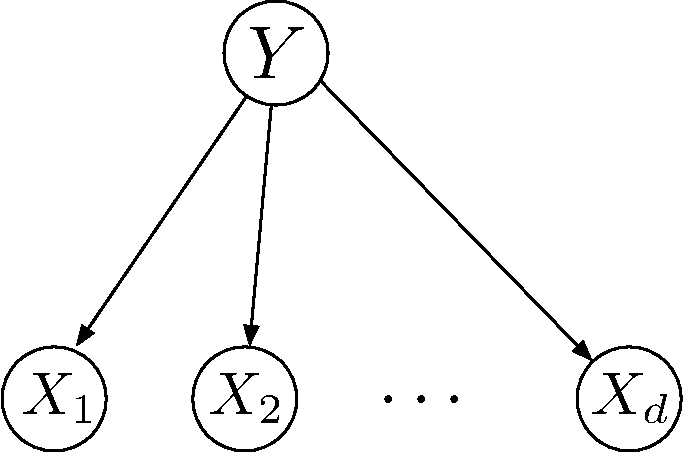
\includegraphics[width=0.3\linewidth]{figures/naivebayesgm}
\end{center}

In this BN, the variable $\mathcal{Y}$ represents some category of interest (e.g., survive versus not survive), and $X_1, X_2, \ldots, X_d$ represent various features of a data point (e.g., age, sex, fare class).  The rules of d-separation tell us that $X_i \condindep X_j~|~Y$ for all $i \neq j$.  For simplicity, we'll assume that $Y$ takes on values from the set $\{1, 2, \ldots c \}$ and each $X_i$ takes on values from the set $\{1, 2, \ldots, r\}$.  Extending your work to the case where each of the random variables takes values from some other discrete set is straightforward.

%Suppose we want to apply the technique of maximum likelihood estimation to the Na\"ive Bayes model.  For training data you are given a training set of input output pairs as $\left (\mathbf{x_1}, y_1 \right),  \left (\mathbf{x_2}, y_2 \right), \ldots, \left (\mathbf{x_n}, y_n \right)$.  Each $\mathbf{x_i}$ represents a $d$ dimensional vector that corresponds to the values of the random variables, $X$, in the BN (e.g., the $j$ the random variable in the BN $X_j$ for the $i$th data point would equal $x_{i,j}$).  Each $y_i$ represents a value for the random variable $Y$ in the bn (e.g., the random variable $Y$ for the $i$th data point would equal $y_i$).

\bes
\item Equation~\ref{eq:mleiidlog} can be written for this model as
\begin{align}
\mathbf{\Theta^\star} &= \argmax_{\Theta} \sum_{i=1}^n \log p(X_1 = x_{i,1}, X_2 = x_{i,2}, \ldots, X_d = x_{i,d}, Y = y_i | \mathbf{\Theta}) \enspace . \label{eq:nbmle}
\end{align}
Using the concept of d-separation on the BN graph for Na\"ive Bayes (the figure above), simplify Equation~\ref{eq:nbmle}.  Hint: you'll want to break apart the big joint probability (the probability of all of the $X_i$'s and $Y$ using conditional independence).

Warning: spoiler alert if you look at part b.
\begin{boxedsolution}
We know that each of the variables in a BN is conditionally independent given its parents.  We can use this result to write the joint probability of all of our random variables the $X$'s and $Y$ in terms of the probability of each conditioned on its parents.
\begin{align}
\mathbf{\Theta^\star} &= \argmax_{\mathbf{\Theta}} \sum_{i=1}^n  \left ( \log p(Y = y_i | \mathbf{\Theta})  + \sum_{j=1}^d \log p(X_j = x_{i,j} | Y = y_i,  \mathbf{\Theta}) \right ) \enspace . \label{eq:nbmle}
\end{align}
\end{boxedsolution}

\item The answer to part (a) is given here to help setup the next part of this question.

\begin{align}
\mathbf{\Theta^\star} &= \argmax_{\mathbf{\Theta}} \sum_{i=1}^n  \left ( \log p(Y = y_i  | \mathbf{\Theta})  + \sum_{j=1}^d \log p(X_j = x_{i,j} | Y = y_i,  \mathbf{\Theta}) \right ) \enspace . \label{eq:nbmle}
\end{align}

Suppose, $\mathbf{\Theta}$ consists of the following parameters.
\bi
\item $\Theta(1), \Theta(2), \ldots, \Theta(c)$ represent the prior probability that $y$ takes on a particular value (e.g., $\Theta(i) = p(Y = i)$).  Note that in order for $\Theta(1), \ldots, \Theta(c)$ to represent a valid probability mass function $\sum_{i=1}^c \Theta(i) = 1$.
\item $\Theta_{j}(k | i)$ represents the conditional probability that feature $X_j = k$ given $Y = i$.  That is $\Theta_{j}(k | j) = p(X_j = k | Y = i)$.  In order for the $\Theta_j(k|i)$'s to represent valid PMFs, $\sum_{k=1}^{r} \Theta_{j}(k | j) = 1$ for all $j$ and $i$.
\ei

Suppose that $\mbox{ycount}(i)$ represents the number of training points where $y = i$ (i.e., $\mbox{ycount}(i) = \sum_{j=1}^n \mathbb{I} \left [y_j = i \right]$ where $\mathbb{I}$ is the indicator function, which returns 1 if the condition is true and 0 otherwise).

Suppose that $\mbox{xcount}_j(k|i)$ represents the number of training points where $x_j = k$ and $y = i$ (i.e., $\mbox{xcount}_j (k|i) = \sum_{u=1}^n \mathbb{I} \left [ x_{u, j} = k, y_j = i \right ]$).

Rewrite Equation~\ref{eq:nbmle} in terms of the $\Theta(i)$'s, $\Theta_{j}(k|i)$'s, $\mbox{ycount}$'s, and $\mbox{xcount}$'s.  Hint: replace summations over the data points with summations over the possible values that the random variables can take on.

Warning: spoiler alert if you look at part c.
\begin{boxedsolution}
TODO: expand this more
\begin{align}
\mathbf{\Theta}^\star &= \argmax_{\mathbf{\Theta}} \left ( \sum_{i=1}^c \mbox{ycount}(i) \log \Theta(i)  \right) +  \left ( \sum_{j=1}^d \sum_{i=1}^c \sum_{k=1}^r \mbox{xcount}_j(k|i) \log \Theta_j(k|i) \right )
\end{align}
\end{boxedsolution}

\item The maximum likelihood equation for the model (the answer to part b) is as follows.
\begin{align}
\mathbf{\Theta}^\star &= \argmax_{\mathbf{\Theta}} \left ( \sum_{i=1}^c \mbox{ycount}(i) \log \Theta(i)  \right) +  \left ( \sum_{j=1}^d \sum_{i=1}^c \sum_{k=1}^r \mbox{xcount}_j(k|i) \log \Theta_j(k|i) \right ) \label{eq:mleparameterized}
\end{align}

Since each various parameters only affect particular terms in these summations, we can break the maximization over the entire parameters space $\mathbf{\Theta}$ into a bunch of separate maximization problems.  For example, the first summation in Equation~\ref{eq:mleparameterized} is only affected by $\Theta(1), \Theta(2), \ldots, \Theta(c)$, therefore
\begin{align}
\Theta^\star(1), \ldots, \Theta^\star(c)&= \argmax_{\Theta(1), \ldots, \Theta(c)}\sum_{i=1}^c \mbox{ycount}(i) \log \Theta(i) \enspace . \label{eq:qmarginals}
\end{align}

One thing to remember about this equation is that not all values of $\Theta(1), \ldots, \Theta(c)$ are permissible.  We know that these parameters have to specify a valid probability mass function, which requires that $\sum_{i=1}^c \Theta(i) = 1$ and each $\Theta(i) \geq 0$. In the language of numerical optimization, these equations are known as \emph{constraints}.

Additionally, for $i$ in the set $\{1, 2, \ldots, c\}$ and $j$ in the set $\{1, 2, \ldots, d\}$
\begin{align}
\Theta_j^\star(1|i), \ldots, \Theta^\star_j(r|i) &= \argmax_{\Theta_j(1|i), \ldots, \Theta_j(r|i)}\sum_{k=1}^r \mbox{xcount}_j(k|i) \log \Theta_j(k|i) \enspace . \label{eq:qconditionals}
\end{align}
For similar reasons to the ones we just stated for  $\Theta(1), \ldots, \Theta(c)$, Equation~\ref{eq:qconditionals} must satisfy $\sum_{k=1}^r \Theta_j(k|i) = 1$  and each $\Theta_j(k|i) \geq 0$ (the reason being, again, that these values must specify a valid PMF).

One way to derive the solution to these constrained optimization problems, is to use the technique of \href{http://tutorial.math.lamar.edu/Classes/CalcIII/LagrangeMultipliers.aspx}{Lagrange Multipliers}.  Here is \href{http://www.cs.columbia.edu/~mcollins/em.pdf}{a walkthrough of using this strategy to solve the equations for the Na\"ive Bayes algorithm} (the proof is in section 4.2).  Instead of having you prove this directly (do prove it if you feel inclined), let's take as given the following theorem.

Suppose $c_1, \ldots c_m$ represent non-negative constants ($c_i \geq 0)$.  Further, suppose $q_1, \ldots q_m$ represents a PMF ($q_i \geq 0$ and $\sum_{i=1}^m q_i = 1$).  If this is true then,

\begin{align}
q^\star_1, \ldots, q^\star_m &= \argmax_{q_1, \ldots, q_m} \sum_{i=1}^m c_i \log q_i \nonumber \\
q^\star_i &= \frac{c_i}{\sum_{i=1}^m c_i} \label{eq:multinomial}
\end{align}

Using the result above, find the optimal values of the parameters of the Na\"ive Bayes model.  In other words, compute $\Theta^\star(1), \ldots, \Theta^\star(c)$ and $\Theta_j^\star(1|i), \ldots, \Theta^\star_j(r|i)$ (for all appropriate values of $i$ and $j$).  Does the result match your intuitions about what the $q$ values should be?

Hint: You should be able to pattern match Equation~\ref{eq:multinomial} to both Equation~\ref{eq:qmarginals} and Equation~\ref{eq:qconditionals}. 

\begin{boxedsolution}
Equation~\ref{eq:qmarginals} can be solved using Equation~\ref{eq:multinomial} in the following way.
\begin{align}
q^\star(i) &= \frac{\mbox{ycount}(i)}{\sum_{j=1}^c \mbox{ycount}(j)}
\end{align}

Equation~\ref{eq:qconditionals} can be solved using Equation~\ref{eq:multinomial} in the following way.
\begin{align}
q_j^\star(k|i) &= \frac{\mbox{xcount}_j(k|i)}{\sum_{u=1}^r \mbox{xcount}_j(u|i)}
\end{align}

TODO: yes, this seems logical...
\end{boxedsolution}


\ees


\end{exercise}

\section{Text Classification with Bag of Words}
Next we'll be applying Na\"ive Bayes to the task of classifying text.

\begin{externalresources}[(45 minutes)]
This will be done in the \href{https://colab.research.google.com/github/mlfa19/assignments/blob/master/Module\%202/03/Assignment_3_Companion_Notebook.ipynb}{Assignment 3 companion notebook}.
\end{externalresources}

\section{The Intelligent Design of Jenny Chow}

This assignment is fully described on the \href{https://canvas.instructure.com/courses/1659968/assignments/12785465?module_item_id=26196347}{Intelligent Design of Jenny Chow Canvas page}.  There is also an alternative described on the assignment page if you can't attend.  Make sure to look at the assignment before going to the play since we are asking you to capture some of your reactions / thoughts so that you can bring them to class on Monday for discussion.

\end{document}
